\documentclass{mproj}
\usepackage{graphicx}

\usepackage{url}
\usepackage{fancyvrb}
\usepackage[final]{pdfpages}
\usepackage{times}
\usepackage{pdfpages}
\usepackage{amsmath}
\usepackage{float}
\usepackage [english]{babel}
\usepackage [autostyle, english = american]{csquotes}
\MakeOuterQuote{"}

% for alternative page numbering use the following package
% and see documentation for commands
%\usepackage{fancyheadings}


% other potentially useful packages
%\uspackage{amssymb,amsmath}
%\usepackage{url}
%\usepackage{fancyvrb}
%\usepackage[final]{pdfpages}

\begin{document}

%%%%%%%%%%%%%%%%%%%%%%%%%%%%%%%%%%%%%%%%%%%%%%%%%%%%%%%%%%%%%%%%%%%
\title{Energy Efficient Knowledge Distribution in Wireless Sensor Networks for Query Analytics}
\author{Kurt Portelli}
\date{\today}
\maketitle
%%%%%%%%%%%%%%%%%%%%%%%%%%%%%%%%%%%%%%%%%%%%%%%%%%%%%%%%%%%%%%%%%%%


\includepdf[pages={1}]{ENDEAVOUR-Acknowledgement.pdf}

%%%%%%%%%%%%%%%%%%%%%%%%%%%%%%%%%%%%%%%%%%%%%%%%%%%%%%%%%%%%%%%%%%%
\begin{abstract}
Systems using Wireless Sensor Networks (WSN) are shaped with the consideration of a great number of factors. These include power consumption, lifetime, network topology, responsiveness and transmission errors. Thus, several research challenges are introduced. We propose a system which lets each network node locally gather knowledge and distribute it amongst its peers. Then, based on this knowledge it evaluates the error and decides whether it should send the updated knowledge or not, minimizing power consumption. Using various techniques we will be querying the learnt shared knowledge and evaluating the accuracy of each to study what the effects of increasing the permissible error are.
\end{abstract}
%%%%%%%%%%%%%%%%%%%%%%%%%%%%%%%%%%%%%%%%%%%%%%%%%%%%%%%%%%%%%%%%%%%

%%%%%%%%%%%%%%%%%%%%%%%%%%%%%%%%%%%%%%%%%%%%%%%%%%%%%%%%%%%%%%%%%%%
\educationalconsent

%%%%%%%%%%%%%%%%%%%%%%%%%%%%%%%%%%%%%%%%%%%%%%%%%%%%%%%%%%%%%%%%%%%

\newpage
%%%%%%%%%%%%%%%%%%%%%%%%%%%%%%%%%%%%%%%%%%%%%%%%%%%%%%%%%%%%%%%%%%%
\section*{Acknowledgements}
I wish to express my sincere gratitude to Dr. Christos Anagnostopoulos for his guidance and expert advice throughout all the various stages of this project. Apart from that I am also thankful to him for making me appreciate even more the subject of data science and machine learning.

Furthermore, I would like to thank my family for all their continuous support in this first year living abroad. 


%%%%%%%%%%%%%%%%%%%%%%%%%%%%%%%%%%%%%%%%%%%%%%%%%%%%%%%%%%%%%%%%%%%
\tableofcontents
%%%%%%%%%%%%%%%%%%%%%%%%%%%%%%%%%%%%%%%%%%%%%%%%%%%%%%%%%%%%%%%%%%%


\chapter{Introduction}\label{intro}
The Internet of Things (IoT) is a rapidly growing area, with it more data is being stored and made accessible which previously has never even been thought possible. IoT is composed of billions of devices that can gather, share information and sometimes even capable of performing operations on this information. IoT devices are physical objects connected with the internet able to share information. This can include anything ranging from smartphones to Radio Frequency Identification (RFID) tags found in everyday products. As more data is made available for anything imaginable that affects our daily lives, opportunities arise for applications that extract this information and make use of it. Y.Wang et al. \cite{distributedEnergyDistribution} state that the smart grid has been recognized as an important form of IoT. It allows a two-way information flow which produces new perspectives in energy management. Making all this information useful is very challenging as it needs to be collected, transferred, stored and made accessible. \cite{intelligentContextualInformation} 

Since these IoT devices are generally wireless, compact and have very limited resources they can be considered as WSNs. REFERENCE ? WSNs are made up of a large number of nodes, which are capable of wireless communication and minimal computation capabilities. \cite{adaptiveDataForwarding} Each sensor node measures the temporal-spatial field of the area around it. These are called the contextual scalar parameters and can be of any form and value, example; humidity, temperature, acidity, etc.. This contextual information is relayed to a "sink", which can referred to as a central node.

In a naive system all these devices generate massive amounts of data which is periodically sent to central node with more computing resources. This in turn, might restructure the data more effectively to be sent to another node or make it available for querying. All this network transfer drains power and as the network size increases this effect is emphasized even more. This has created a need and opportunity for machine and statistical learning algorithms.\cite{LargeScaleOnlineLearning} According to L.Bottou et al.\cite{LargeScaleOnlineLearning} these technological improvements have outrun the exponential evolution of computing power. Thus, we must rely more on on-line learning algorithms to process these large amounts of data with comparatively less computing power.

The vision of IoT is to allow any device to be continuously connected sharing its knowledge about the surroundings. Machine learning then uses this stream of data to deduce results, infer new knowledge, reason about contextual events or make assumptions. The possibilities for such systems are endless, taking, for instance, the case of thermometers in rooms next to each other and based on previous information the temperature of various rooms can be predicted based on the temperature of adjacent ones.

\section{Problem Synopsis}
One of the factors in IoT systems is the collection of contextual information from certain sources in an IoT environment.\cite{intelligentContextualInformation} IoT devices communicate in an ad-hoc manner with the Central nodes, also known as collectors to send information. The objective of each collector is that it has the latest up-to-date information/context. This would allow the IoT system to further process the context and make use of it, example environmental monitoring.

In this IoT environment the IoT devices are not able to communicate directly together due to the limited resources, so instead they communicate with the collectors. Even if each device has an infinite power supply, a naive system which periodically transmits the context is not feasible especially as the network grows in size. Collectors would become overloaded with messages from all devices and incur a performance degradation as network size increases. Transmitting wireless messages is very costly and in most cases IoT devices run on limited battery power. These devices need to make intelligent decisions whether to send data or not to conserve battery power and increase their lifetime. In this naive system there is no concept of knowledge, thus withholding data would result in the collectors having gaps of knowledge.

Once the collectors have access to the context of the connected devices, they need to make it available for querying. A naive system stores all the data items inside the context for each device. This would result in a very resource hungry collector due to the huge amount of processing and storage capabilities it would need to support. C.Anagnostopoulos \cite{intelligentContextualInformation} states that the contextual sensor data exhibits high complexity, dynamism, accuracy, precision and timeliness. This is due to the huge volumes, interdependency relationships between devices and continuous updates performed in real-time. From this statement he then argues that "an IoT system should not concern itself with the individual pieces of contextual sensor data: rather, context should be intelligently collected and interpreted into a higher, domain relevant concept."\cite{intelligentContextualInformation}

Using this concept, instead of having access to all the raw data, collectors would contain multiple intelligent contexts. This raises the challenge on whether for each query there exists an optimal set of intelligent contexts that increase the accuracy. In other words it opens the opportunity for ensemble learning \cite{dietterich2002ensemble}. This means that we cannot guarantee to find the best hypothesis (intelligent context) that gives the best accuracy from all contexts. Ensemble learning tries to intelligently choose contexts and assign weight depending on their likelihood of providing the best result. Hence, it aims at reducing the bias and variance of the learning algorithms used to construct the context.\cite{dietterich2002ensemble}

The research challenge we will be looking at is the building of an energy efficient network which minimises power consumption while simultaneously minimising transmission error. Furthermore, we will investigate the use of ensemble learning on the local contexts to achieve more accurate queries. This system must make use of very little computing resources to maximise its lifetimes while at the same time support scalability and real-time querying for environment monitoring.

\section{Project Aims}
We argue that instead of directly sending the contextual information, devices should locally learn their context using machine learning algorithms and then transmit this knowledge. If we transmit the local model to the central node each time it is updated then we would not save any power consumption. Thus, we go a step further and set up the notion of a  permissible error, which allows the local and central models to have a limited amount of discrepancy. This allows us to avoid unnecessary transmissions which do not "teach" the collector any valuable knowledge, and in turn reduce the power consumption. Altering the permissible error should determine the percentage of messages being sent, thus directly affecting power consumption.

We will be using on-line linear regression to learn the context of each device with real-time constraints. Primarily we will be investigating how the error discrepancy between devices and collectors affect battery consumption and network lifetime. Secondly we will study how altering this error discrepancy has an effect on the querying accuracy of the collectors.

The primary objectives for this project may be defined as follows:
\begin{itemize}  
\item Obtain a clear understanding on how IoT systems operate and what they try to achieve.
\item Implement On-line machine learning and clustering algorithms. In particular, we will be focusing on a 3-dimensional implementation.
\item Build a system capable of simulating a real-life IoT system containing collectors and devices. We will be using the U-Air \cite{air-quality-inference-meets-big-data} dataset, which contains air quality data from real-life stations in Beijing and Shanghai.
\item Integrate the capability of transmitting both raw context and knowledge (with a flexible degree of error) to investigate energy efficiency of our implementation.
\item Evaluate the query accuracy performance of both naive system and our implementation.
\end{itemize}

\section{Document Outline}
The content of this report is organized into the following chapters:
\begin{itemize}
\item \textbf{Chapter 2} provides the reader with the background knowledge required for understanding the basic principles and algorithms behind this work. In particular, we introduce the general theory behind on-line algorithms, linear regression and normalization.
\item Afterwards, in \textbf{Chapter 3} we analyse the related work in this field to provide us with the required knowledge to improve upon what there already is.
\item \textbf{Chapter 4} describes our major contributions to the research challenges, namely network efficiency and ensemble learning.
\item In \textbf{Chapter 5} we describe the major design and implementation decisions of our contributions and simulation system.
\item \textbf{Chapter 6} contains the evaluation and performance analysis of our work.
\item Lastly in \textbf{Chapter 7} we identify possible future extensions, and conclude the presented work.
\end{itemize}

\chapter{Preliminaries}
In this chapter, we present an overview of the concepts and base principles we mention and make use of in our work. We develop a system which deals with a continuous data stream and thus, has to use specialized algorithms which treat each data item individually without storing past data items. Various algorithms are used which extract knowledge from each individual sensor by minimizing loss and then quantize the input.

\section{On-line Algorithms}
According to M.Karp \cite{Karp} an on-line algorithms is one which receives a sequence of requests and performs an immediate action to each request. These are useful in situations where decisions must be made without any future knowledge. Their effectiveness is measured by the comparing them with their off-line (batch) counterparts. In this dissertation we make use of well known common techniques already proven to work.

\subsection{K-Means}
The K-means algorithm attempts to find K representatives (centroids) of a data set in such a way as to best represent the data. \cite{onlinekmeans} Although it is algorithmically simple, it still manages to be relatively robust and give close to optimal results on a wide range of data sets. Its disadvantage is that one has to predefine K. Furthermore, the initial K centroids chosen have a drastic effect upon the clusters chosen. The first k inputs initialize the codebook vectors (centroids) $m_j,j=1,...,k$. The rest of the inputs $x^t \in X$ are used for the update function.
\begin{equation}
\label{eq:chooseCluster}
i \longleftarrow arg min_j \parallel x^t - m_j \parallel
\end{equation}
\begin{equation}
\label{eq:updateCluster}
m_i \longleftarrow m_i + \eta (x^t - m_i)
\end{equation}
Equation \ref{eq:chooseCluster} finds the closest centroid to the input. Then the closest centroid is updated as shown in equation \ref{eq:updateCluster} depending on the learning rate defined by $\eta$. A large $\eta$ enhances accuracy but makes $m_i$ oscillate. Therefore to reach convergence one needs to use a small or decaying $\eta$.

\subsection{Adaptive Resonance Theory (ART)}
\label{sec:artExplanation}
ART\cite{art} is another unsupervised learning algorithm similar to k-means. It does not require the number of clusters to be predefined before hand. Instead one has to define \textit{vigilance} which represents the degree of similarity between points. An data item $x^t \in X$ is a member of a cluster $m_j$ only if the distance between them is less than vigilance. Similar to the K=means procedure, once $m_j$ is chosen, equation {eq:updateCluster} is used to update the centroid. If no centroid satisfies this constraint, then a new cluster is created. This allows a better flexibility but has the disadvantage of creating an infeasible and unpredictable amount of clusters in certain situations.

\subsection{Linear Regression}
\label{linearregression}
Once it is proven that there is a statistically significant correlation between two variables, linear regression allows us to make predictions about one variable based only on the other variable. The relationship between these two values must be linear, else this technique would not be able to model the data accurately.

To perform this supervised learning we must first start by defining the hypothesis example the linear function \ref{eq:hypothesis}.
\begin{equation}
\label{eq:hypothesis}
h_\theta(x) = \theta_0 + \theta_1x_1 + \theta_2x_2
\end{equation}
The $\theta_i$'s represent the weights of the linear function, thus, determining the mapping between X and Y. Let $x_0=1$, we then rewrite equation \ref{eq:hypothesis} to a more compact form represented by equation \ref{eq:hypothesisShort}.
\begin{equation}
\label{eq:hypothesisShort}
h(x) = \sum_{i=0}^{n} \theta_ix_i = \theta^Tx
\end{equation}
For this hypothesis to be useful, the $\theta$ parameters need to be trained to fit a particular dataset. Conceptually the closest $h(x)$ is to Y, the better we are at representing the data. Thus, we define the cost function equation \ref{eq:costFunction} which measures the total discrepancy for each input $x^{(i)}$ with output $y^{(i)}$.
\begin{equation}
\label{eq:costFunction}
J(\theta) = \frac{1}{2}\sum_{i=1}^{m}( h_\theta(x^{(i)})-y^{(i)})^2
\end{equation}
Naturally, we would like to choose a theta which minimizes the error. One such technique which does this is the gradient descent rule. It calculates the gradient of the error and takes a step proportional to the negative gradient. To achieve this we need to use the partial derivative of equation \ref{eq:costFunction}. For all $\theta$ the update rule then becomes equation \ref{eq:updateDerivative}. This update rule is called least mean squares (LMS) and it has a very interesting property. The magnitude of the update is proportional the the error. This means that the greater the error, the steeper the descent towards the minima.  After completing the derivative we are left with the complete equation \ref{eq:batchUpdate}. This has to be repeated for each $\theta$ until convergence. Meaning until we reach the best possible theta values.
\begin{equation}
\label{eq:updateDerivative}
\theta_j := \theta_j - \alpha\frac{\partial}{\partial\theta_j}J(\theta)
\end{equation}
\begin{equation}
\label{eq:batchUpdate}
\text{Repeat until convergence: (For each j) }
\theta_j := \theta_j - \alpha\sum_{i=1}^{m}(y^{(i)}-h_\theta(x^{(i)}))x_j^{(i)}
\end{equation}
One might argue that with this iterative approach we might get stuck at a local minima instead of finding the optimal minima. In this particular scenario J is a convex quadratic function, meaning it has only one minima. Thus, gradient descent will always converge at the global minima assuming $\alpha$ is not too large.

\subsubsection{Multivariate Stochastic Gradient Descent}
The previous algorithm is called batch gradient descent as for each update step it uses all all the training set. This would not be feasible to compute especially as the dataset size increases. Another issue would be that previous data items have to be stored, and this is not always possible. In fact we will be using the more lightweight and on-line version called stochastic gradient descent. In batch gradient descent we go through all the data set for a single update step while when using equation \ref{eq:stochUpdate} we start making progress right away. We use this update rule for each new training item we encounter. This in fact has the tendency of getting close to $\theta$ much faster than batch gradient descent, however it may never converge and instead keep oscillating around the minimum. The reason it is called multivariate is that we will be using multiple inputs (more than one $x$) to get $y$.

\begin{equation}
\label{eq:stochUpdate}
\text{(For each j) }\theta_j := \theta_j + \alpha(y^{(i)}-h_\theta(x^{(i)}))x_j^{(i)}
\end{equation}

\subsection{Mean and Variance}

\section{Probability Distribution Function}

\section{Normalization}
We use the standard score \cite{normalization} to normalize the dataset. This is done by subtracting each item $x$ by the mean and then dividing it by the standard deviation of the dataset as shown in equation \ref{eq:standardScore}. Performing this normalization allows us to better understand the results as it gives a meaning to a raw value. Figure \ref{fig:zscore} demonstrates the distribution of $z$, a negative value means that x was less than the mean. Furthermore, the magnitude of this value represents the distance from the mean in terms of standard deviation.
\begin{equation}
\label{eq:standardScore}
z= \frac{x - \mu}{\sigma}
\end{equation}
\begin{figure}[H]
\caption{Standard score normalization \cite{normalization}}
\label{fig:zscore}
\centerline{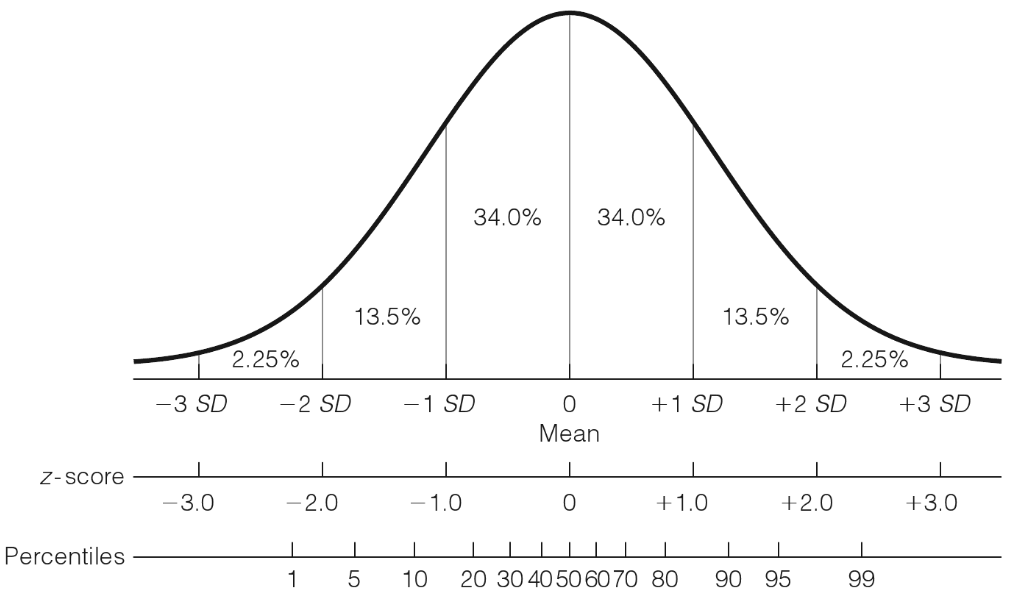
\includegraphics[scale=0.4]{zscore}}
\end{figure}

\section{K Nearest Neighbours (KNN)}
\label{sec:knnExplanation}
KNN \cite{knn} is a straightforward classification technique, in which given an input it is able to classify it to certain class. As the name implies it takes the closest K neighbours and depending on the majority of their classes it determines the class of the input. Figure \ref{fig:knn} demonstrates KNN ($K=3$) while classifying X using a data set containing 3 different classes. In this case input X is classified as Red due to the fact that the majority of its 3 closest neighbours are Red.
\begin{figure}[H]
\caption{At KNN=3, Input X is classified as Red}
\label{fig:knn}
\centerline{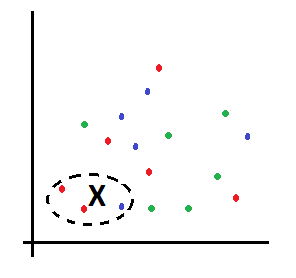
\includegraphics[scale=1]{knn}}
\end{figure}

\chapter{Literature Review}

\chapter{Contributions}
In this chapter we discuss our major contributions with the aim of improving WSNs. More specifically how we can increase network efficiency, which extends the devices' life time. We shall delineate a strategy for creating knowledge from the raw context, by locally learning the context in real-time using on-line stochastic gradient descent. Based on this knowledge, we then decide whether it is worth it to transmit data or not.
Additionally we look into how we can minimize the error when querying the knowledge found inside the collectors.
\section{Model Description}
We start by considering an IOT system composed of sensor nodes and a collector depicted in figure \ref{fig:sn}. Sensor nodes are only capable of communicating with collectors. Collectors can then be queried or in turn be considered as sensor nodes and connected to larger tree structure, creating a larger more complex network. Resources are reserved for communication, processing and data sensing. Message transmission consumes much more energy when compared to the processing and data sensing tasks. \cite{teen} Thus, we argue that if we let the nodes continuously sense data and only transmit this information when it is essential, we could create a more energy efficient network. A.Manjeshwar et al. \cite{teen} states that this is possible because sensor networks are "data centric", meaning that data is requested based on certain attributes and not requested for a certain node. The requirements of each WSN change according to the application as some nodes might be static while others mobile. When nodes are adjacent to each other certain similarity might occur, thus, data can be aggregated. A common query in these systems is for example which area has humidity $<$ 10\% rather than what is the humidity of area $X$. We can use this knowledge to our advantage and define a system that can minimize the number of messages transmitted while at the same time still provide accurate results from queries.

\begin{figure}[H]
\caption{Model Example}
\label{fig:sn}
\centerline{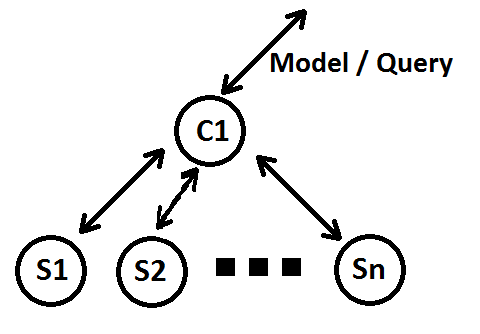
\includegraphics[scale=0.5]{sensornetwork}}
\end{figure}

\section{Network Efficiency}
Consider a sensor node $i$ which receives a new data item $p(t)$ at time $t$. Our system needs to decide whether it is worth transmitting this new data or not. To achieve this, we create a local model based on linear regression. The function we compute will enable us to predict the error and have a quantifiable way of deciding whether transmitting $p(t)$ is worth it or not. Since each sensor node has limited resources, both computational and storage limitations we use on-line stochastic gradient descent to calculate the regression line. A full detailed description of on-line stochastic gradient descent can be found in the Preliminaries chapter, section \ref{linearregression}. Using this algorithm we avoid storing a history of values and instead we consider each new data item alone, then discard it. 

Each sensor $i$ locally and incrementally builds its own model from sensing the pairs $(x,y)$. After a period of learning, each sensor sends its model parameters to a centralized concentrator. Take for instance weights $w=[w_0,w_1,w_2]$ from equation \ref{eq:modelParams}. 

\begin{equation}
\label{eq:modelParams}
f[i](x) = w_0 + w_1x_1 + w_2x_2
\end{equation}

Once a sensor $i$ has sent its local model $F[i](x)$ to the concentrator, then for every new $(x,y)$ data pair it receives, it is capable of updating the local model and deciding of whether to update the concentrator model as well. For every new $(x,y)$ the $w$ parameters might change when compared to the original model sent previously to the concentrator. Sensor $i$ upon receiving an $(x,y)$ pair it updates the model and predicts the output $y*$ from its current local $f[i](x)$ with parameters $w'$ and then measures locally the error $e* = |y-y*|$. If the model has not significantly changed the 'obsolete' model in the concentrator will experience a similar error. Sensor $i$ keeps a copy of the original w (obsolete model in concentrator), thus, knows exactly the error the concentrator would experience. Hence, let us denote this error from the original local model as $e\# = |y - y\#|$ where $y\#$ is the prediction of y when involving the original (obsolete) model $f[i](x)$ with parameter $w$. At that time, sensor $i$ has two prediction errors: $e*$ and $e\#$. The $e\#$ is the error that concentrator would experience if the same input $x$ was used.

\begin{equation}
\label{eq:differenceError}
De = |e* - e\#|
\end{equation}

Using Equation \ref{eq:differenceError} we are able to get the discrepancy in error between the 2 models. We then use the condition $De > THETA$ to determine whether it is worth it to update the obsolete model or not. A $THETA=0$ would mean that the local and concentrator model would be synchronized at all times. On the other hand when we increase $THETA$ we transmit less messages, thus, increase network efficiency. This would also mean we are now susceptible to an increase in error between the 2 models. Figure \ref{fig:nea} shows a simplified flowchart of the algorithm just described in this section.


\begin{figure}[H]
\caption{Sensor Node Flowchart}
\label{fig:nea}
\centerline{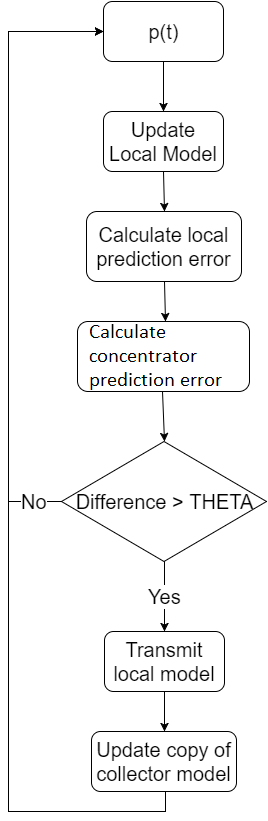
\includegraphics[scale=0.5]{NetworkEfficiencyAlgorithm}}
\end{figure}

\section{Ensemble Learning}
The previous section explains our algorithm which increases network efficiency by transmitting less messages to the concentrator. This is done by altering $THETA$ which determines the acceptable error. An increase in network efficiency means that sensors working on battery power can last longer without the need of recharging. As previously mentioned the purpose of an IOT system is that it can be queried from the "root" (concentrator). In this section we aim to extend the model defined in the previous section to reduce the error at the concentrator level.

Naively the concentrator would have all the $(x,y)$ data pairs and when queried with an arbitrary $x$, it can directly search in its storage for the best match and return $y$ accordingly. In our model the concentrator collects a function $f[i](x)$ for each sensor $i$ which simulates the data collected. The ideal scenario is that when the concentrator receives query $x$, it would also know which function $f$ it should use to predict $y$. Unfortunately, in a real-life scenario this is not possible as we would not know which sensor $x$ is related to.

One solution is that the concentrator proceeds with averaging the prediction results from all the collected functions $f[i](x)$. The concept behind averaging all the predictions ensures that the over-estimates and under-estimates are balanced out. We argue that this might not always produce an optimal result and it can further be improved. There exists scenarios where an input $x$ is not observed by some of the functions, thus, leading to poor predictions. Take for instance the case where multiple thermometers are sparsely placed around a building. Sensors next to a kitchen might in general observe temperature readings in a higher range than sensors placed outside. Given a high temperature $x$, would it be better to average the predictions from all the sensors or use only the kitchen sensors?

With this concept in mind, we extend the previous model and add data representatives of the input space. Using these data representatives, the system would be able to determine whether a function $f$ is familiar to the query $x$ or not. To elect data representatives we use an on-line clustering algorithm which quantizes the input space. We used both K-Means and ART which are described in detail in the Preliminaries chapter; section \ref{sec:knnExplanation} and \ref{sec:artExplanation}. When a data pair $(x,y)$ is used to update the model, we also update the centroids in the clustering algorithm. The centroids are transmitted to the concentrator along with local model.

The concentrator now has the necessary information to determine what the input space of each function is. When query $x$ is submitted, the concentrator can select the functions which have data representatives in the vicinity. The assumption is that these functions were generated from values similar to the query, thus, have more reliable knowledge.

\section{Adding the "Reliability" variable}
Right now the concentrator is able to select which functions to use based on the distance between query $x$ and centroids. We believe the distance alone might not be sufficient enough to describe the input space of each function. Our intuition is that some sensors produce more accurate results than others. To study this, we performed an analysis on the Beijing Air Quality dataset \cite{air-quality-inference-meets-big-data} and trained a regression model for each sensor. We then isolated 2 sensors at a time and predicted the y using 3 different methods; 

\begin{itemize}  
\item Endogenous error - In this test we predict y of sensor $i$ using regression function $f(i)$.
\item Exogenous error - In this test we predict y of sensor $i$ using regression function $f(i+1)$.
\item Fusion error - In this test we predict y of sensor $i$ using both regression functions $f(i)$ and $f(i+1)$ and then take the mean.
\end{itemize}

\begin{figure}[H]
\caption{Endogenous, Exogenous, Fusion errors}
\label{fig:functionsErrors}
\centerline{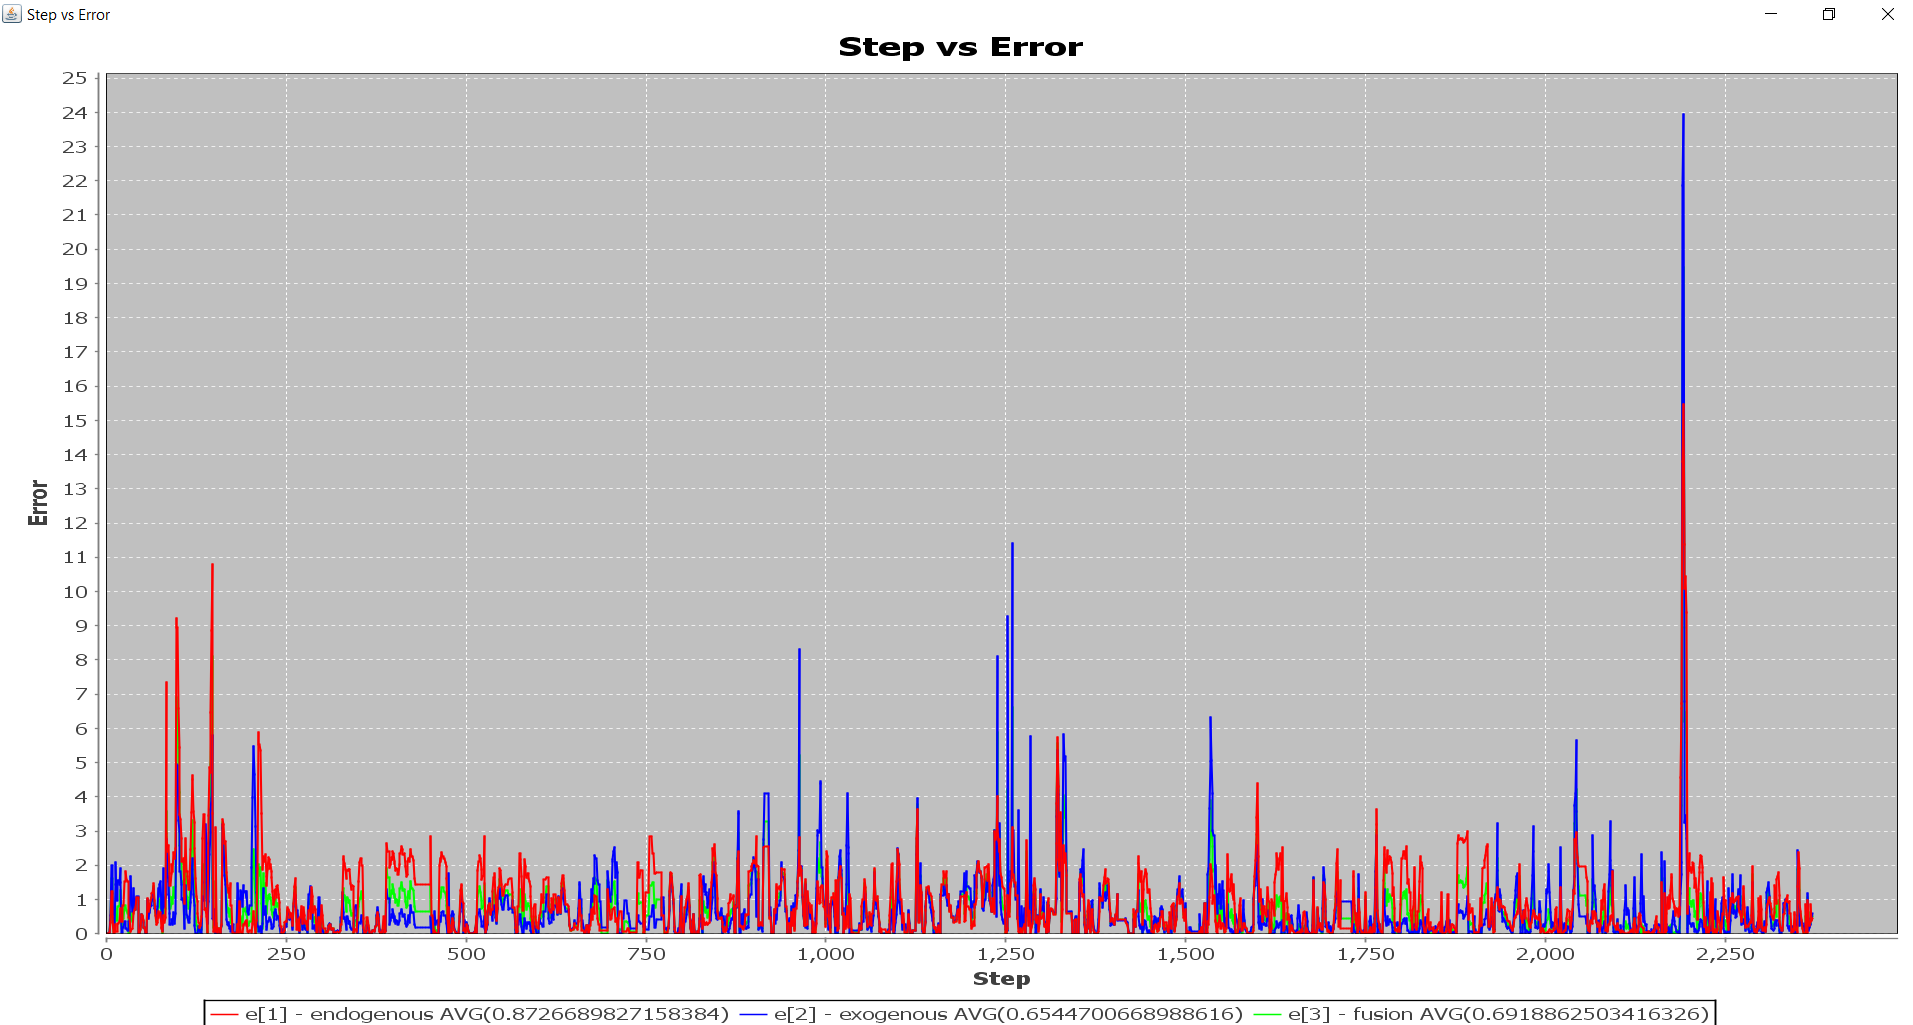
\includegraphics[scale=0.4]{e1e2e3}}
\end{figure}

Figure \ref{fig:functionsErrors} shows one of the studies done using the first 2 sensors. In this case using just the regression model from another sensor (exogenous) proved to more accurate rather than using its own model. The reason might be because some centroids are more popular, while others yield less error in certain situations. This is were ensemble learning is useful, and we can leverage the knowledge the concentrator has about every sensor attached to it. The concentrator should try to choose a subset from all the sensors to provide more accurate results. Centroids which are frequently updated tend to have a higher average error due to the frequent updates to the regression model. Hence, we should consider the number of times each centroid is used to determine the popularity. Thus, along with each centroid we include an error value and number of times used.

\begin{equation}
\label{eq:ourEquation}
weight=\frac{e^{-distance} + e^{-error} + used}{3}
\end{equation}

\begin{figure}[H]
\caption{$e^{-x}$ Function}
\label{fig:e-x}
\centerline{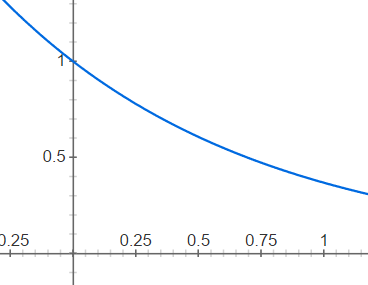
\includegraphics[scale=0.4]{e-x}}
\end{figure}

Equation \ref{eq:ourEquation} defines how we assign a weight to each centroid in relation to a given query. Once we sort the centroids in descending order according to their weight, we would get an amalgamation of the 3 properties; closest, lowest error and most popular. Note, that the values of \textit{used} are normalized between 0 and 1 so as to makes use of the exponent function shown in figure \ref{fig:e-x}. As distance and error approach 1 (highest possible due to normalization), the exponent function inverts them and gives them a low value. On the other hand as \textit{used} approaches 1 we would like to give it a higher weight, thus we leave it as is.

\chapter{Design and Implementation}
In the previous chapter we laid the theoretical groundwork and intuitions of our system, and now we proceed to examine how they were implemented into fully working algorithms. We begin by explaining the dataset that we shall be using and how it is structured as it will affect the design of the system. Afterwards, we explain how our system capable of simulating an IoT environment was designed and implemented. This includes the network aspect and statistics gathering. We then explain in detail our contributions regarding network efficiency and ensemble learning mentioned in the previous chapter.

\section{Dataset}

\section{Network Architecture}

\section{Query Analytics}

\chapter{Evaluation and Case Study}

\section{Data Set}

\section{Error Allowance vs Messages Sent}

\section{Probability Distribution Functions}

\section{Query Validation}

\chapter{Conclusion}\label{conclusion}

\section{Achievements}

\section{Future Work}

\section{Final Remarks}

\appendix % first appendix

\chapter{First appendix}

\section{Section of first appendix}

\chapter{Second appendix}

\bibliographystyle{plain}
\bibliography{mproj}
\end{document}
